% v1.0 released 28th January 1994

\documentclass[a4paper]{article}
\usepackage[margin=1.0in, top = 1.2in, bottom=1.4in]{geometry}
%\usepackage{amsmath}
\usepackage[fleqn]{amsmath}
\usepackage{mathtools}
%\usepackage{natbib}
\usepackage{graphicx}
\usepackage{mathrsfs}
%\usepackage[usenames,dvipsnames]{color}
%\usepackage{aas_macros}
\usepackage{amssymb}
\usepackage{multirow}
%\usepackage{comment}
%\usepackage{subfigure}
\usepackage{hyperref}
%\usepackage{epstopdf, dcolumn}
\usepackage{color}
%\DeclareGraphicsExtensions{.eps}

\usepackage{fancyvrb}

\newcommand{\Rom}[1]{\uppercase\expandafter{\romannumeral #1}}
\newcommand{\rom}[1]{\lowercase\expandafter{\romannumeral #1}}
\newcommand{\Msun}{\mathrm{M_\odot}}
\newcommand{\hl}[1]{{\color{blue}#1}} 
%%%%%%%%%%%%%%%%%%%%%%%%%%%%%%%%%%%%%%%%%%%%%%%%

\begin{document}
\title{\Huge Pack Allocation Algorithms}

%\begin{document}

\date{\today}


\maketitle

\label{firstpage}
\section{Description of Problem}

Allocate the number of bakery products $m$ to a finite types of packs with sizes
(number of units) $V_i$ ($i=1, 2, ... n$). The allocation result can be described as $a_i$ ($i=1, 2, ... n$), which means the required number of pack $i$ is $a_i$.  An optimal solution is to minimize total number of required packs
$$B = \sum_{i=1}^n a_i,$$
subject to
\begin{itemize}
   \item $v_i > 0$ is a positive integer
   \item $a_i \geq 0$ is a non-native integer
   \item all products are allocated: $\sum_{i=0}^n a_i V_i = m$, where $m$ is the quantity of products to be allocated
\end{itemize}
The total price of the products can be calculated as
$$P = \sum_{i=1}^n p_i a_i,$$ where $p_i$ is the price of pack $i$.
\section{Algorithms}
This problem is NP-hard. A exhaustive search would be computationally expensive. I have therefore proposed a first-fit greedy approximation algorithm. the greedy algorithm, is verified using an exhaustive search.

\subsection{Greedy Heuristic}
This greedy heuristic always try to allocate the items to largest possible pack. If this is a reminder, try to allocate the reminder to next smaller pack until the smallest. If still not divisible, remove one large pack and and add the number of items $V_i$ it to the reminder and try again. The greedy algorithm is run in a recursive manner:
\begin{enumerate}
\item Sort the packs by their sizes, so that $V_0 > V_1 > .. V_n$.
\item Start from the largest pack $i=0$. Let the reminder $r$ equals $m$
\item Divide $r$ by $V_i$, let $a_i$ = quotient and $r$ = reminder
\item If $r = 0$, return the results
\item If $r > 0$, try next smaller pack $i = i + 1$, go to Step 3
\item If still not divisible, remove 1 current pack and repeat Step 3 - 6 until $a_i = 0$
\item If still $r>0$ at the end. The products are not allocable by these packs.
\end{enumerate}


\subsection{Exhaustive Search}
The exhaustive algorithm is also implemented in a recursive manner. For all $i=1, 2, .., n$, try $a_i = 0, 1, ...,\mathrm{reminder}[r/V_i]$. At the end of each step, subtract allocated items from the reminder $r$, this reduces the upper bound of the next loop.

\section{Validation and Test} 
 
\subsection{Example Test Cases}
The greedy heuristic is tested against the test cases from the specification. See Table {\ref{tab:example-test}} for the test cases.
\begin{table}
\label{tab:example-test}
 \caption{Example test cases}
 \centering
 \begin{tabular}{| c | c | c | c | c |}
 \hline
        product code & quantity ($m$) & pack sizes ($v_i$) & allocation ($a_i$) & test result\\
 \hline
 		VS5 & 10 & [5, 3] & [2, 0] & pass \\
 		MB11 & 14 & [8, 5, 2] & [1, 0, 3] & pass\\
 		CF & 13 & [9, 5, 3] & [0, 2, 1] & pass\\
  \hline
 \end{tabular}
\end{table}

\subsection{Verification}

The completeness the greedy heuristic is validated with the exhaustive algorithm. Two criteria are tested for $m$ in $1, 2, ... 100$.
\begin{itemize}
\item If the exhaustive finds at least a solution, the greedy heuristic also finds one. \item If the greedy heuristic doest not find a solution, no solution can be found by exhaustive search.
\end{itemize}

Specially, under configuration in Table {\ref{tab:example-test}}. I have also verified that the greedy heuristic is able to find one of the optimal allocation solutions.


\section{Performance}

\subsection{Accuracy}

The greedy method is a heuristic, it allocates the products to packs from large to small and return the allocation results immediately if it has fond one. For example, These are two optimal allocation for MB11 configuration [8, 5, 2], which are [1, 0, 3] and [0, 2, 2]. The greedy method is able to find the first one, as it allocates 1 to the larger pack $v_0=8$.

Under more complex pack configuration, the greedy method may not give the best solution. for example, If $V$ = [6, 5, 2] and $m=10$. The heuristic gives [1, 0, 3]. The exhaustive search can find the optimal allocation [0, 2, 0].

Under current pack configuration as shown in Table {\ref{tab:example-test}}. The greedy heuristic is able to find one of the optimal allocation solutions.

\subsection{Time complexity}
The run time of the exhaustive algorithm increases almost exponentially with the quantity in the order. When $m=1000$, it requires $\sim 36s$ to complete the run based on my machine, which is not applicable and the greedy approximation heuristic becomes a must. In a simple pack configuration, the time complexity of the greedy heuristic $\sim O(1)$.

\begin{figure*}
    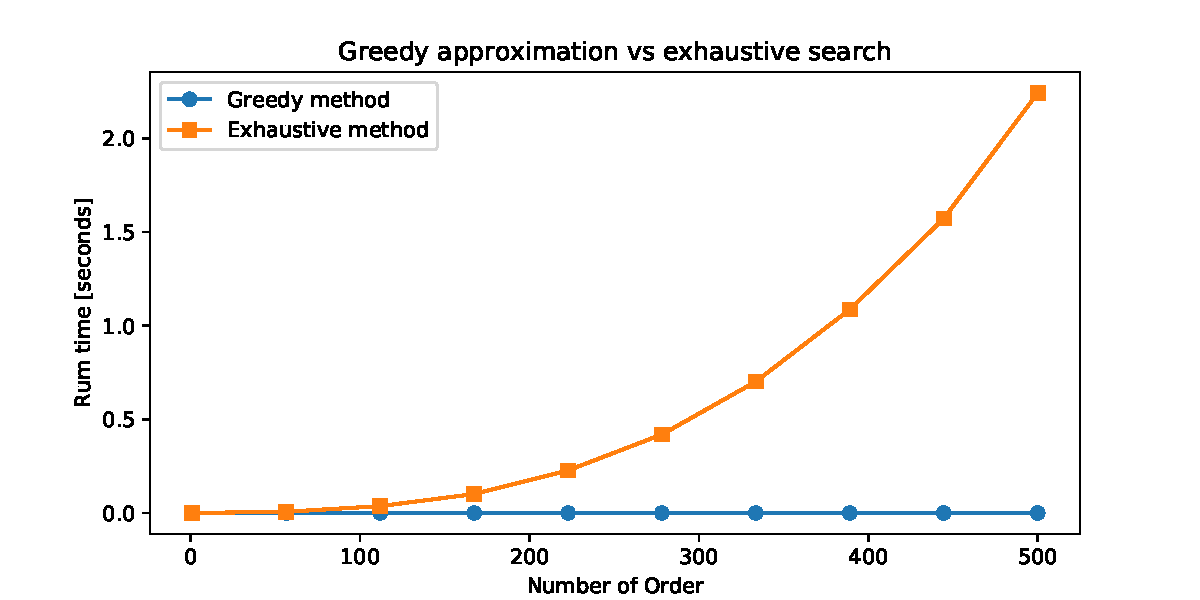
\includegraphics[width=\textwidth]{./comparison.pdf}
    \caption{The speed performance of the greedy approximation and the exhaustive search}
\end{figure*}

\end{document}
